\subsection{General}\label{chapter_GENERAL}

As mentioned in the foreword, the goal of this student project is to design and implement a state space controller for a quadrocopter. But what is a state space controller? And what at all is a quadrocopter?

The first question is too complex to give a short overview. So it is answered in detail in chapter \ref{chapter_THEORY}.
But it is possible to give a short overview over the quadrocopter, although it is described in detail in chapter \ref{chapter_PHYSICAL_MODEL}.

A quadrocopter is a four-engined aircraft, similar to a helicopter with four rotors. The four rotors are placed at the four 'edges' of the aircraft and allow the quadrocopter to start and land vertically. 

\begin{center}
	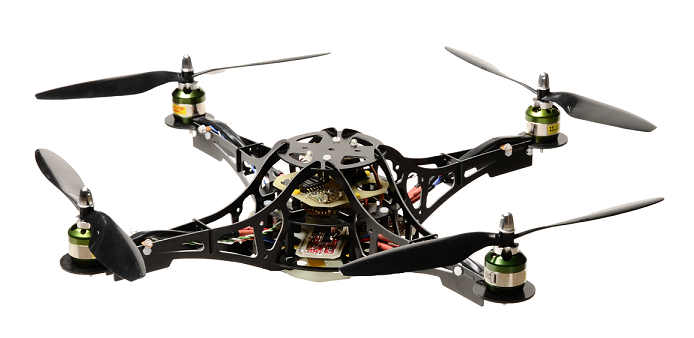
\includegraphics[width=1.00\textwidth]{03_Grafiken/QuadrocopterImage.png}
\end{center}

To achieve horizontal movement, the quadrocopter gets pitched, and by crossover speed up and slowdown of the propellers, it is possible to achieve vertical rotation.
The quadrocopter, this project is based on, gets steered by a four-way remote control. The pilot is able to control the horizontal angles, the vertical rate of rotation and the average speed of the propellers. So the quadrocopter definetely needs an interface, to interpret the commands of the remote control and calculate the engine speed of every motor/propeller. In other words - an embedded controller is needed.
State of the art is a cascaded PI controller, which works fine. Nevertheless it is reasonable to design and implement this mysterious state space controller, to see if it works as well as the PI controller or even better. Besides, a state space controller has some advantages over a classical PID controller.

The development of the controller is an engineering process, that needs structured proceeding, so the next step of this paper is a view on the project management and the structure of this document.